\documentclass[pdftex,12pt]{article}

\usepackage[utf8]{inputenc}
\usepackage[english]{babel}
\usepackage[english]{isodate}
\usepackage[parfill]{parskip}
\usepackage[pdftex]{graphicx}
\usepackage{todonotes} % \todo{note} \listoftodos
\usepackage{microtype}
\usepackage{titling}
\usepackage{booktabs}
\usepackage{multirow}
\usepackage{hyperref}
\usepackage{float}
\usepackage{longtable}

% Commands
\newcommand{\HRule}{\rule{\linewidth}{0.5mm}}

\title{Maxwell Katz for Dummies}
\author{Harrison J Katz}
\date{\today}

\begin{document}
\pagenumbering{Roman}

% Title Page
\begin{titlepage}
    \begin{center}
        \ % starts a paragraph so tex is happy
        \textsc{\huge \thetitle}\\
        \textsc{An Instruction Manual}\\[1em]
        \HRule \\[1em]

        \begin{figure}[h!]
            \centering
            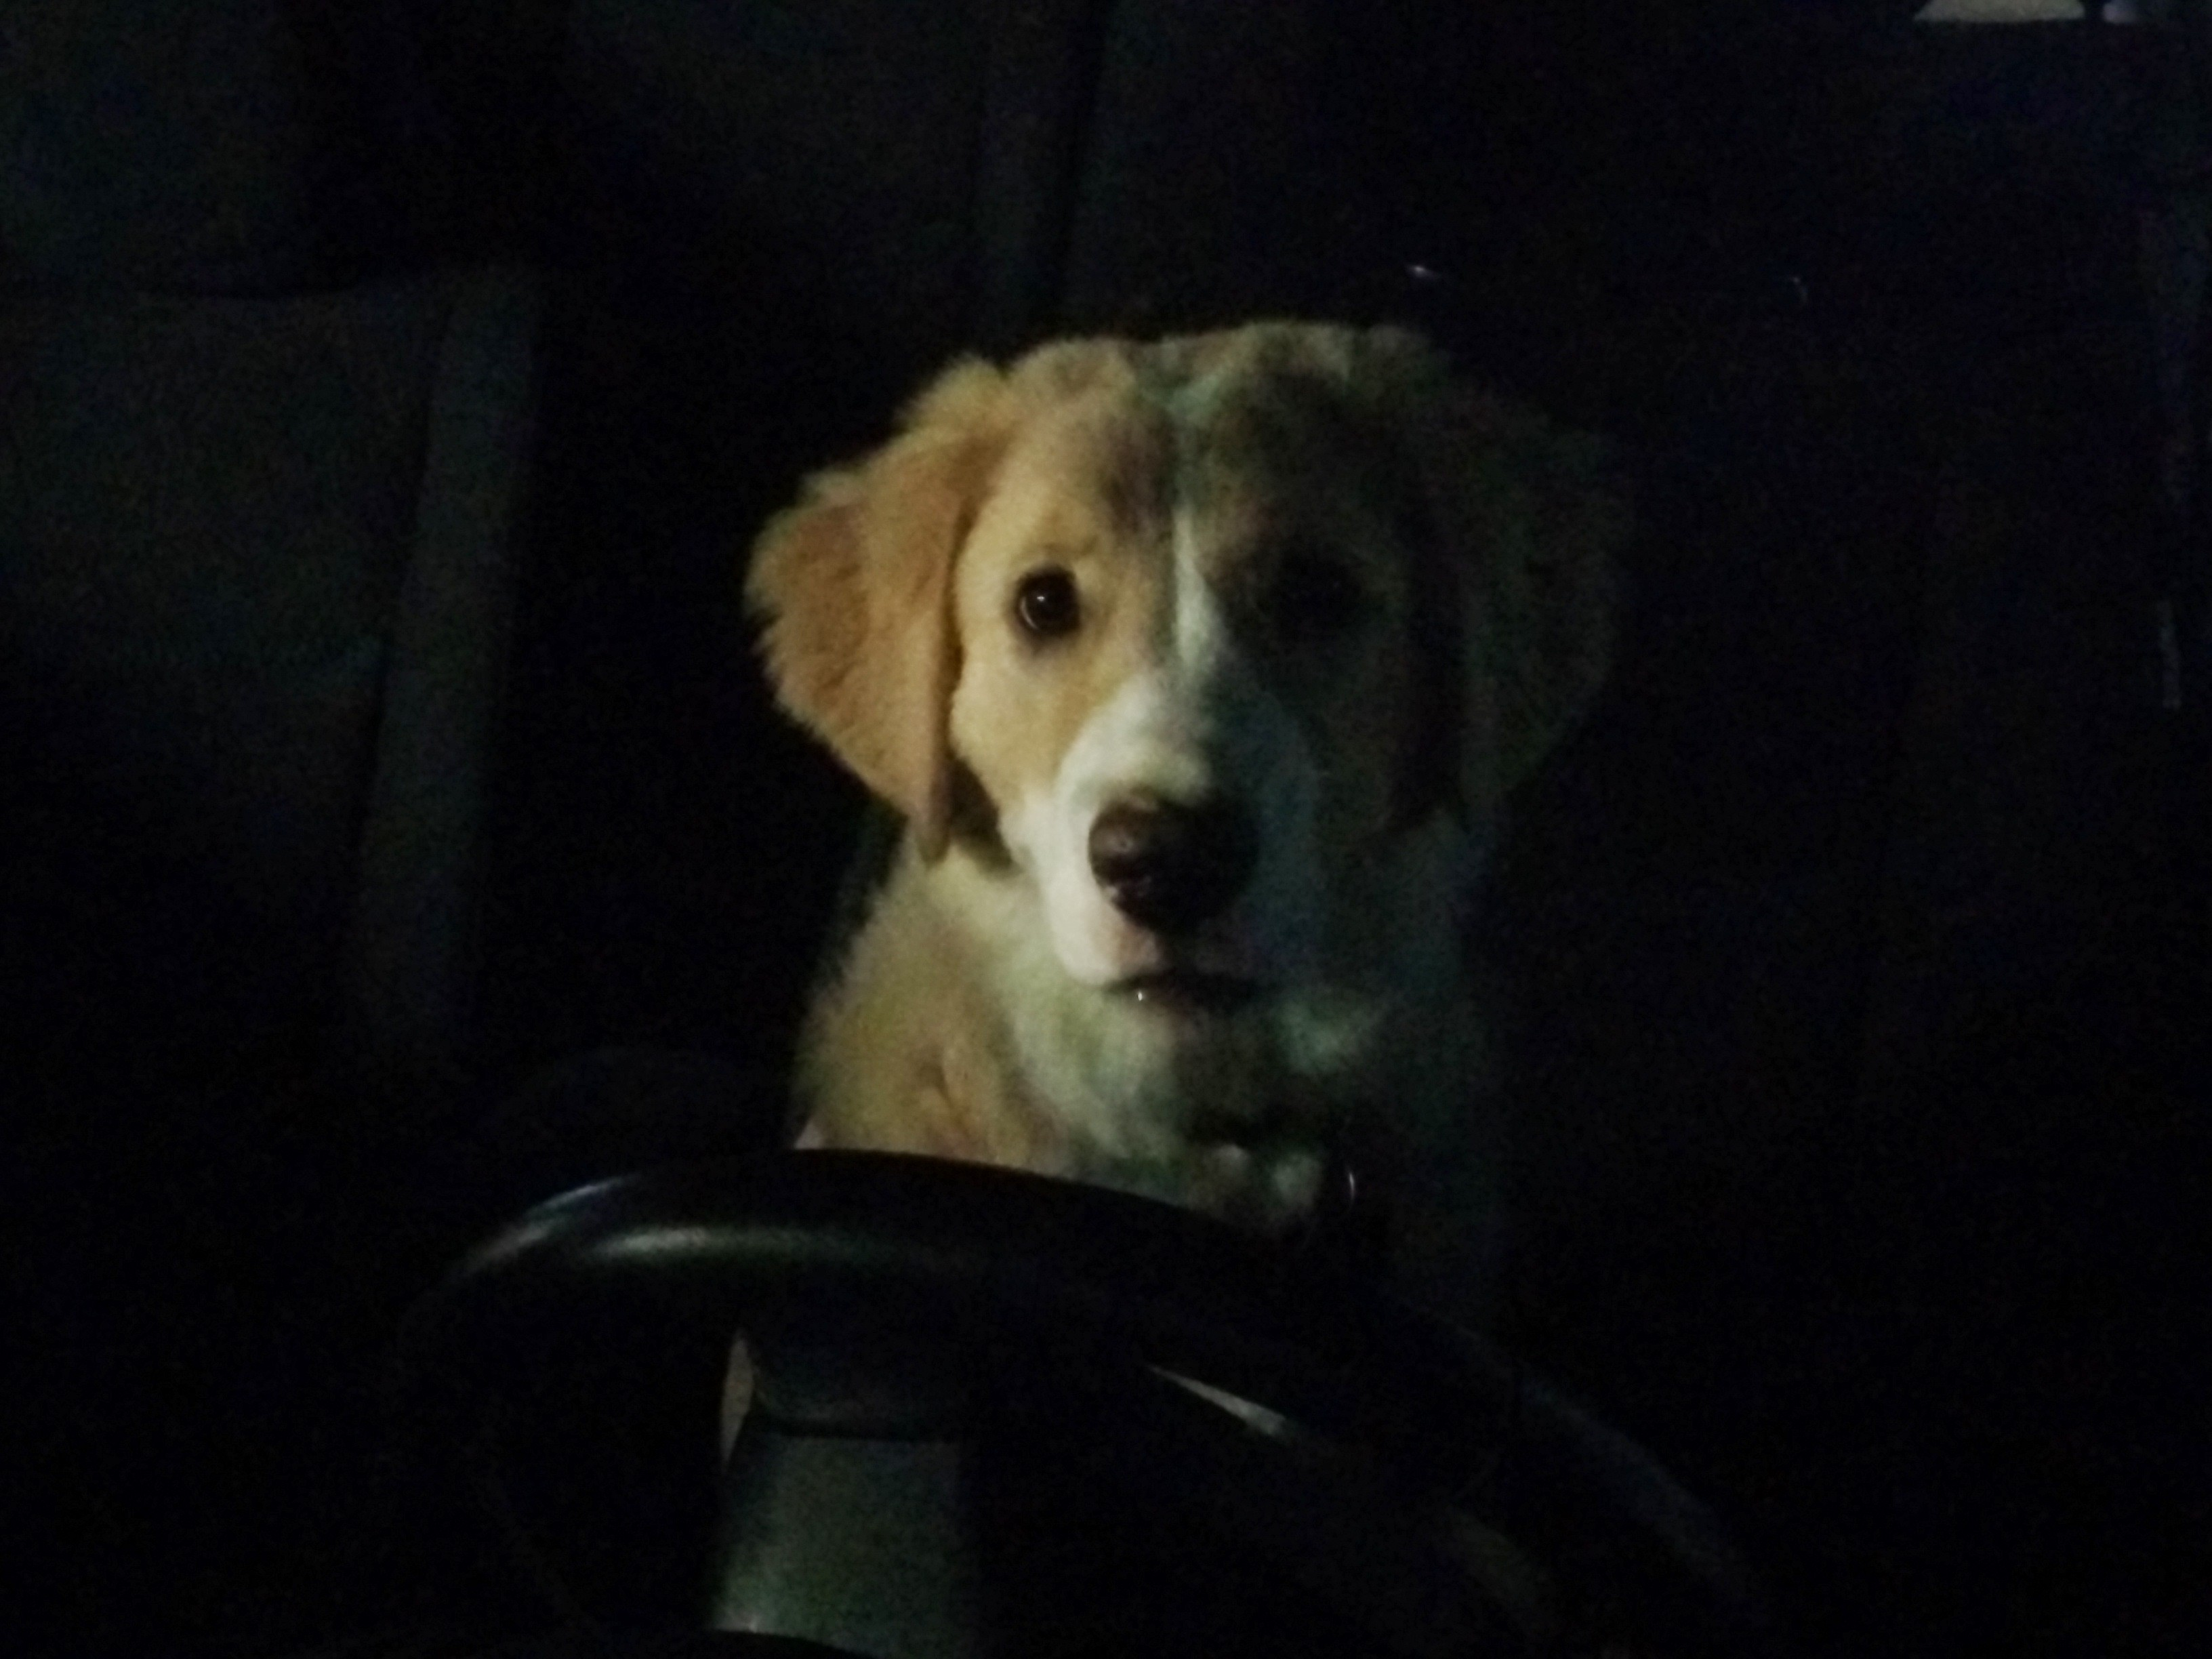
\includegraphics[width=.75\textwidth]{./images/max/title.jpg}
            \caption{Maxwell learning to operate a motor-vehicle.}
            \label{fig:max_title}
        \end{figure}

        % Bottom of the page
        \vfill
        {
            \large \theauthor \  --- \large \thedate
        }

    \end{center}
\end{titlepage}


% Contents
\newpage
\tableofcontents
\todo{Information, emergency, contacts, medicines}
\todo{Schedule, eating, walks, play}
\todo{Training, commands, disciplen, rewards}
\todo{What to do if...}

% Figures
\newpage
\listoffigures

% Document
\newpage
\pagenumbering{arabic}

\section{Introduction}

So, you've been wrangled into babysitting a dog. Not just any dog though, Max.
\emph{Sigh.} What are you going to do? Maxwell Katz (no middle name) is a
rambunctions, destructive, incorrigible goofball, yet he will tug at your
heartstrings with his lovable face and ears. What should you do? What does he
eat? \emph{Oh no!} What does he do for fun? What should I do in the case of
emergency? This may seem like a lot to handle, but fear not, all of this and
more will be answered in this manual.

\newpage
\section{Emergency Information}

\begin{table}[H]
    \begin{longtable}{@{}ll@{}}
        \toprule
        \multicolumn{2}{c}{Pet Information}                                                                              \\ \midrule
        Name          & Maxwell Katz                                                                                     \\
        Answers to    & "Max!" "Maxwell" "*whistle* Come here!"                                                          \\
        Breed         & Golden Retriever / Great Pyrenees                                                                \\
        Color         & Golden White (Toasted Marsh-mellow)                                                              \\
        Date of Birth & January 9th, 2014                                                                                \\
        Health Issues & N/A                                                                                              \\
        Allergies     & Chocolate                                                                                        \\
        Other         & Has 2 extra toes, a trait of Pyrenees                                                            \\ \midrule
        \multicolumn{2}{c}{Owner Information}                                                                            \\ \midrule
        Name          & Harrison John Katz                                                                               \\
        Phone \#      & 706.801.5289                                                                                     \\
        Email         & hjkatz03@gmail.com                                                                               \\ \midrule
        \multicolumn{2}{c}{Emergency Contact}                                                                            \\ \midrule
        Name          & Laura Katz                                                                                       \\
        Relation      & Mother of Harrison Katz                                                                          \\
        Phone \#      & 706.612.4572                                                                                     \\
        Email         & ldkatz38@gmail.com                                                                               \\ \midrule
        \multicolumn{2}{c}{Veterinary Information}                                                                       \\ \midrule
        Name          & Peachtree Hills Animal Hospital                                                                  \\
        Phone \#      & 404.812.9880                                                                                     \\
        Address       & \multirow{3}{*}{\begin{tabular}[c]{@{}l@{}}3106 Early Street\\ Atlanta, GA\\ 30305\end{tabular}} \\
                      &                                                                                                  \\
                      &                                                                                                  \\
        Website       & \url{http://www.peachtreehillsvet.com}                                                           \\
        Email         & info@peachtreehillsvet.com                                                                       \\
        Hours         & Monday-Friday, 8am-6pm                                                                           \\
        Emergency     & \url{http://www.peachtreehillsvet.com/emergencies}                                            
    \end{longtable}
    \label{tab:information}
\end{table}

% Todos
\newpage
\listoftodos

\end{document}
